% -*- LaTeX -*-
% -*- coding: utf-8 -*-
%
% michael a.g. aïvázis <michael.aivazis@para-sim.com>
% (c) 2010-2020 all rights reserved
%

\section{components}

% --------------------------------------
\begin{frame}
%
  \label<1>{frame:altar-application-pedigree}
%
  \frametitle{The structure of the driver}
%
  \vskip -3ex
%
  \only<1>{
    \begin{center}
      
\includegraphics[width=1.0\textwidth]{application-class}
    \end{center}
  }
%
  \only<2>{
    \begin{center}
      
\includegraphics[width=1.0\textwidth]{application-altar}
    \end{center}
  }
%
  \only<3>{
    \begin{center}
      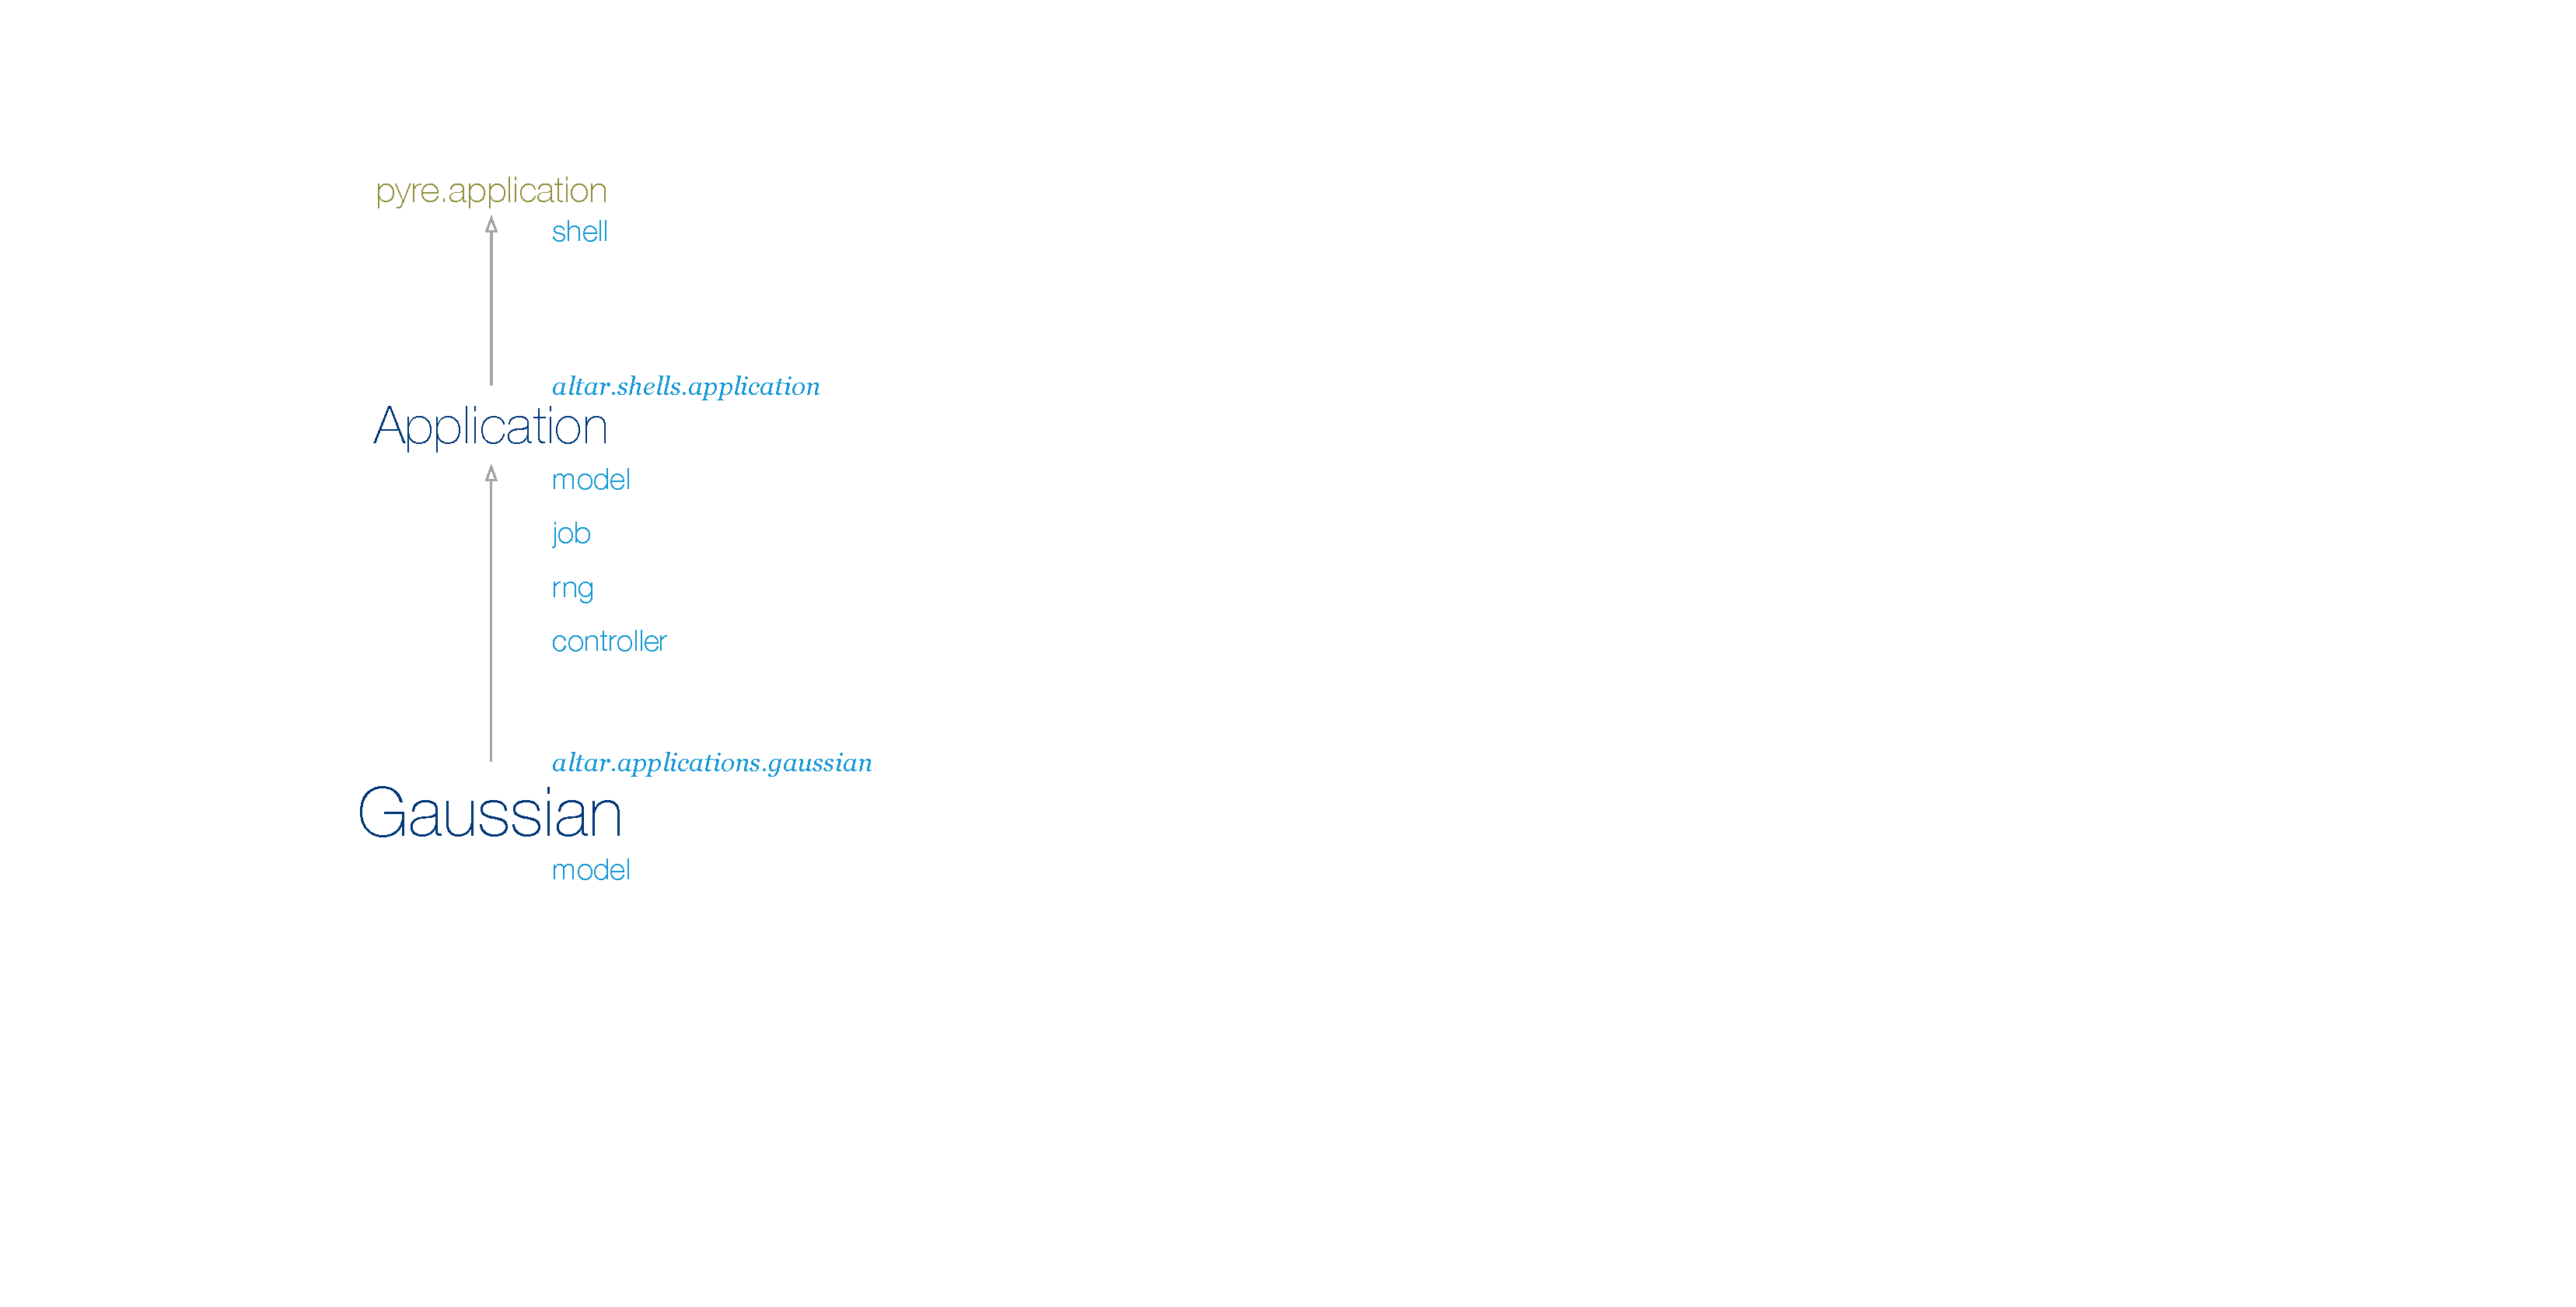
\includegraphics[width=1.0\textwidth]{application-pyre}
    \end{center}
  }
%
  \only<4>{
    \begin{center}
      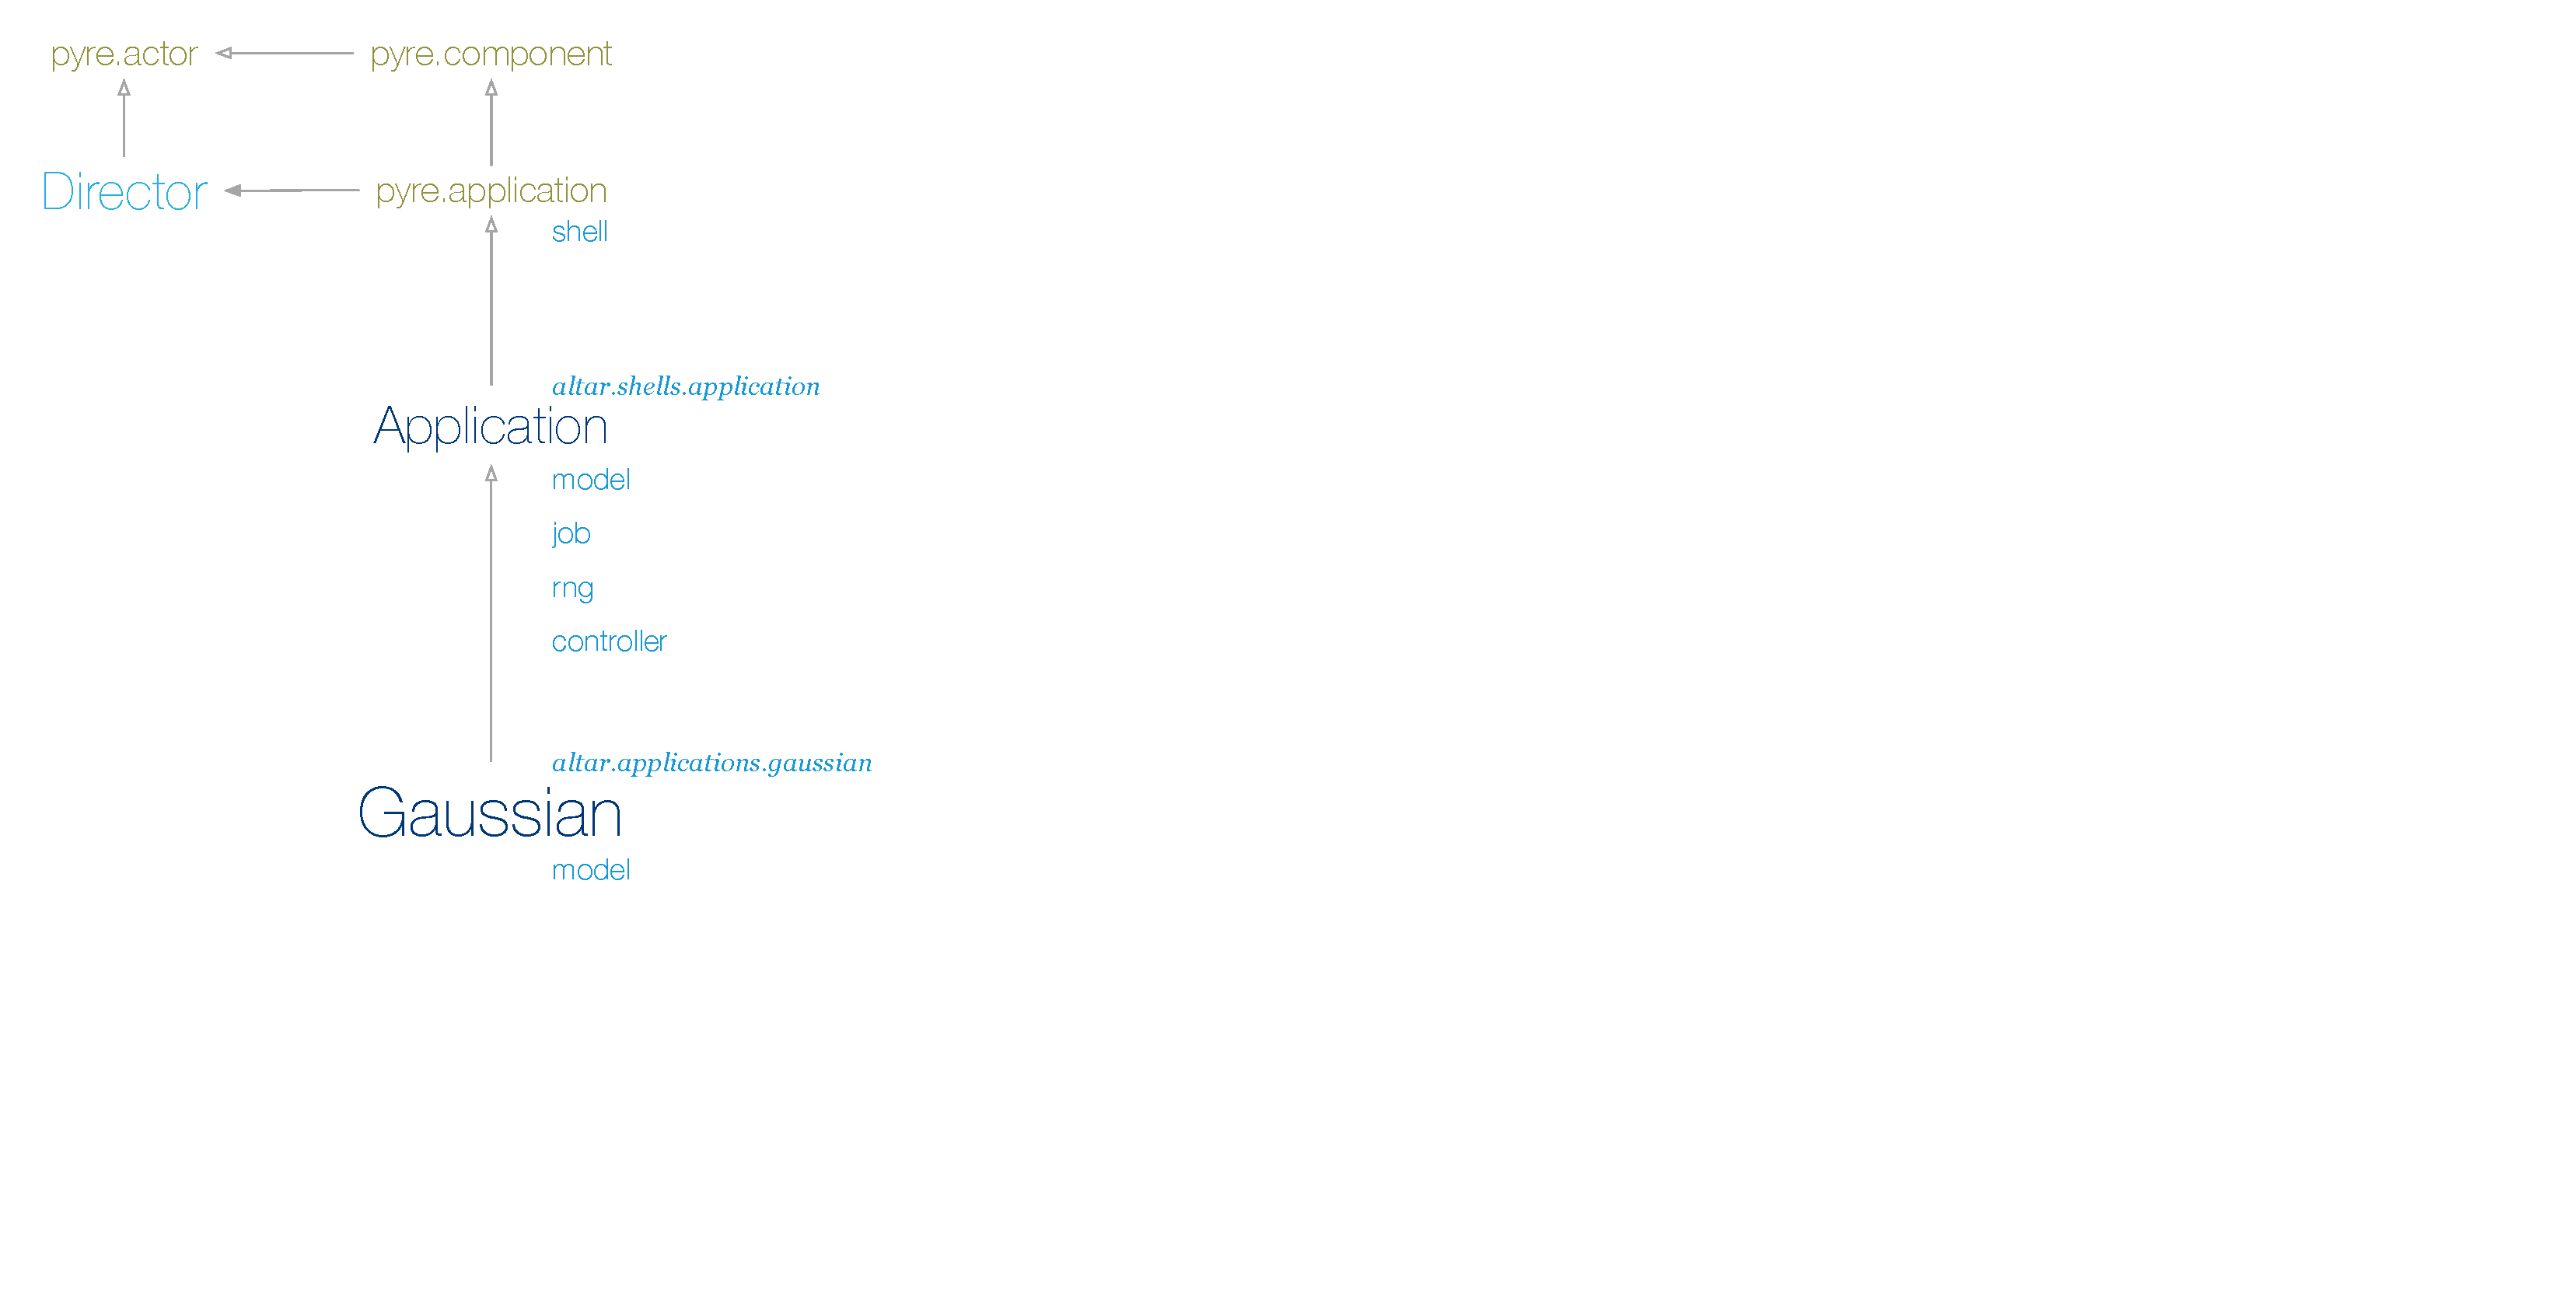
\includegraphics[width=1.0\textwidth]{application-pedigree}
    \end{center}
  }
%
  \only<5>{
    \begin{center}
      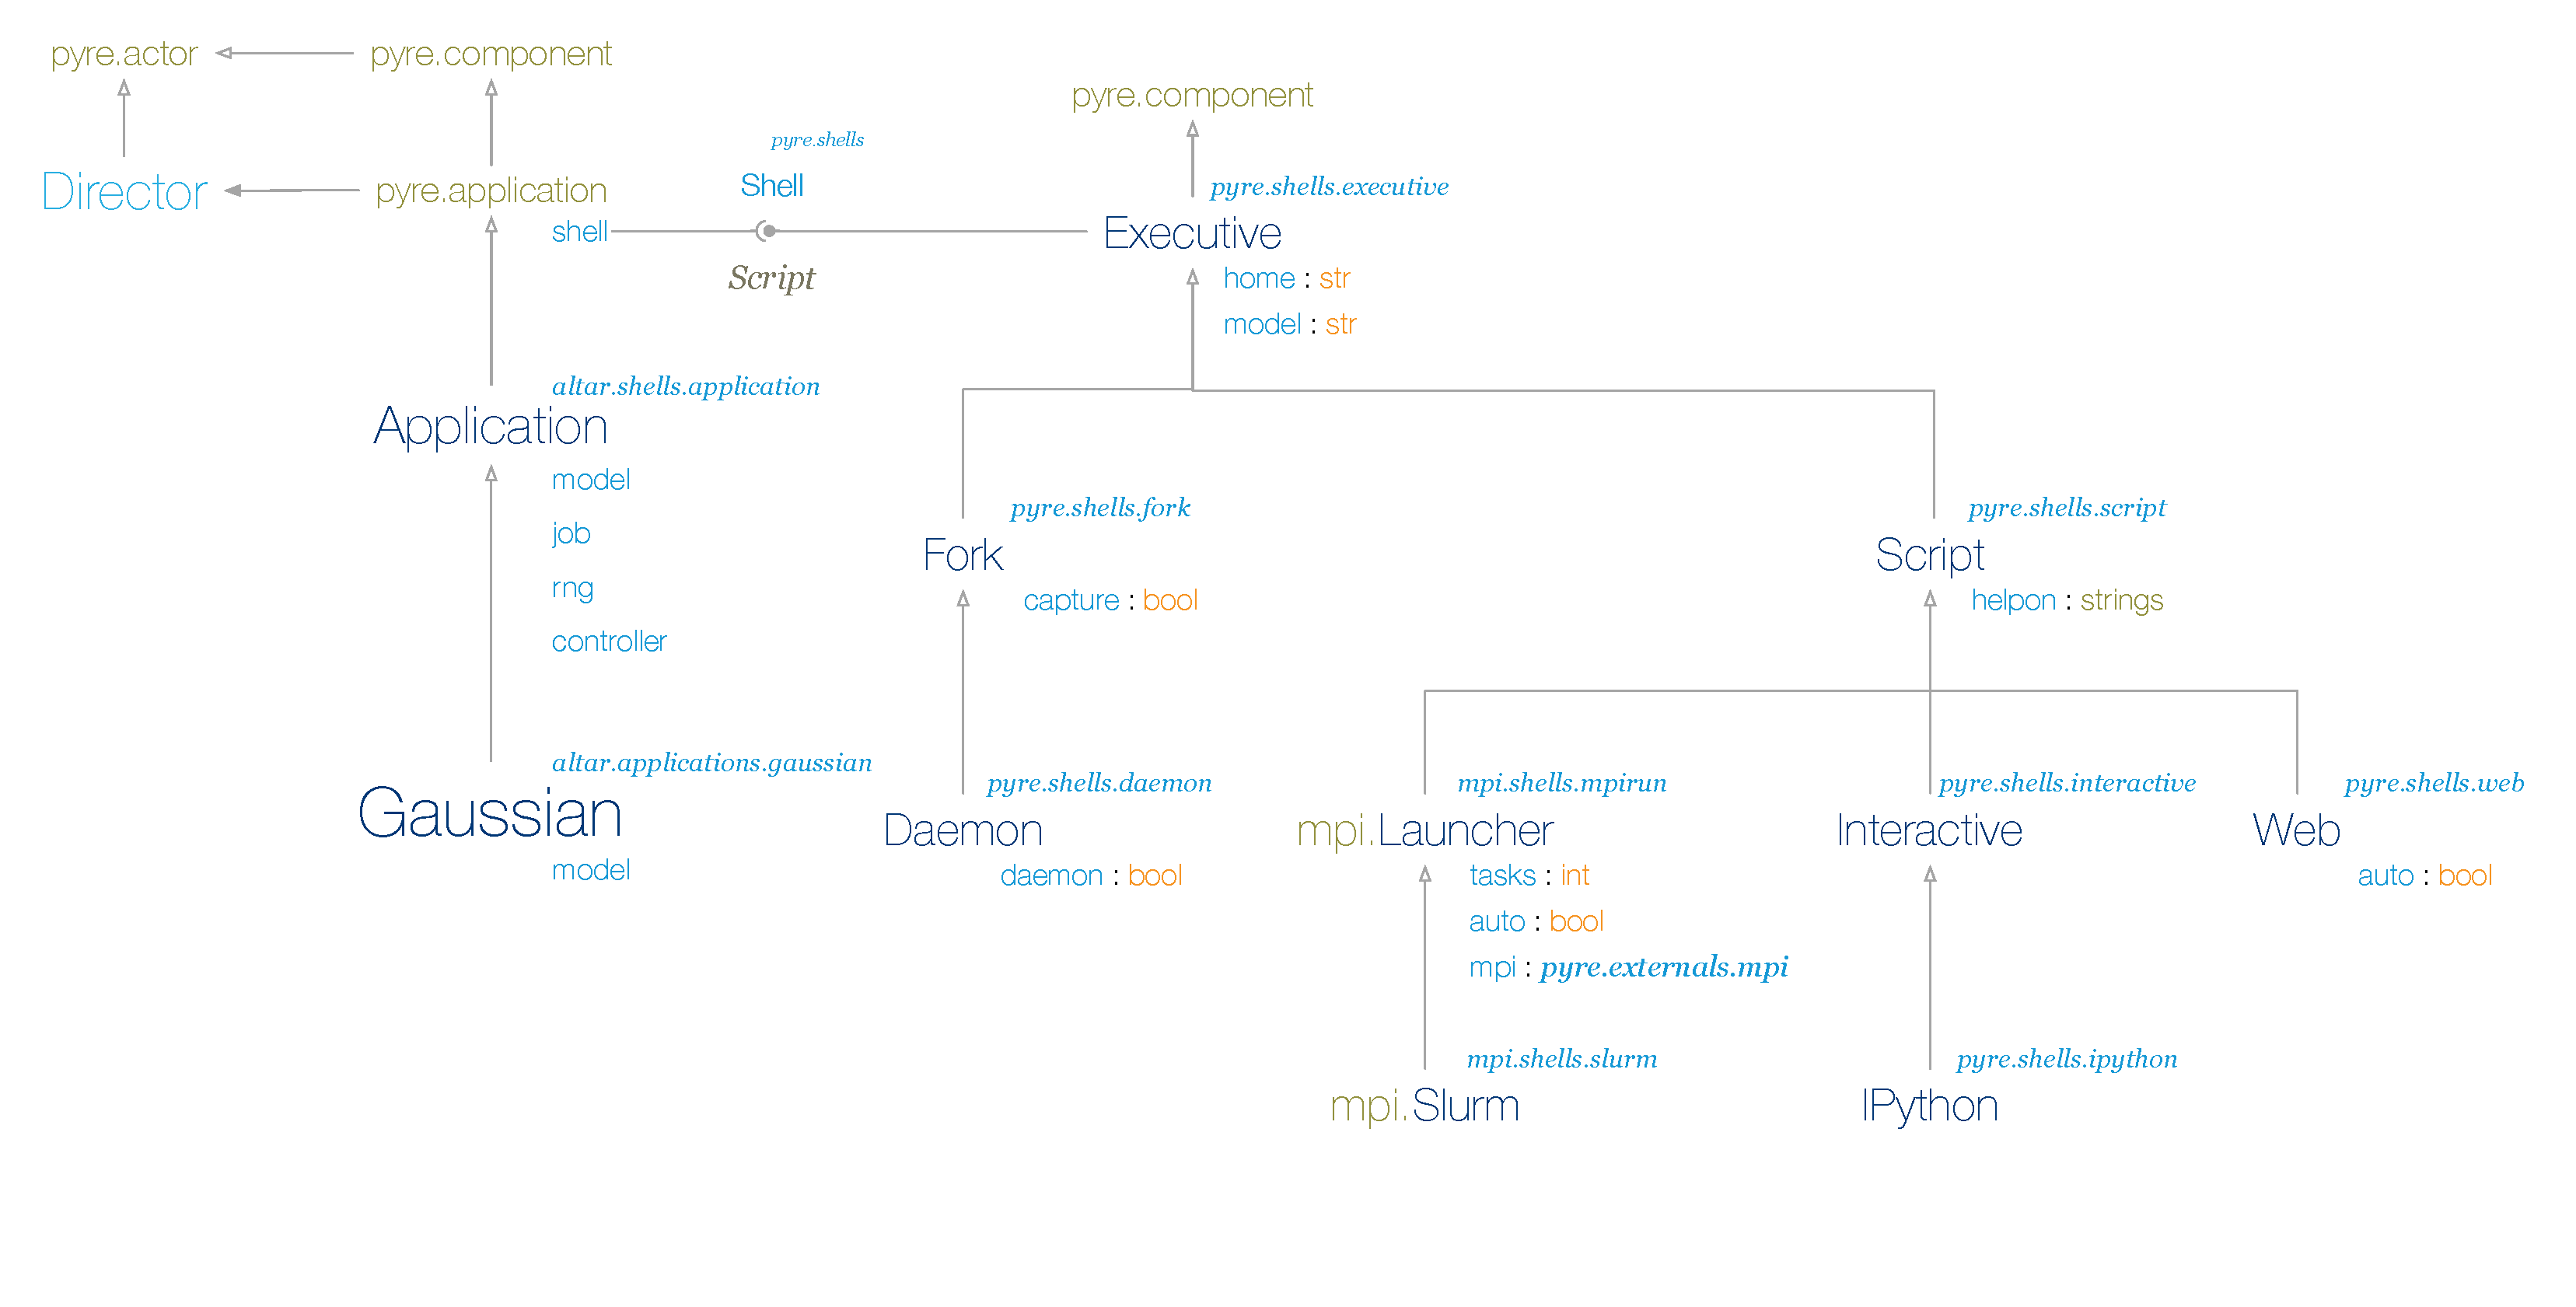
\includegraphics[width=1.0\textwidth]{application-shell}
    \end{center}
  }
%
  \only<6>{
    \begin{center}
      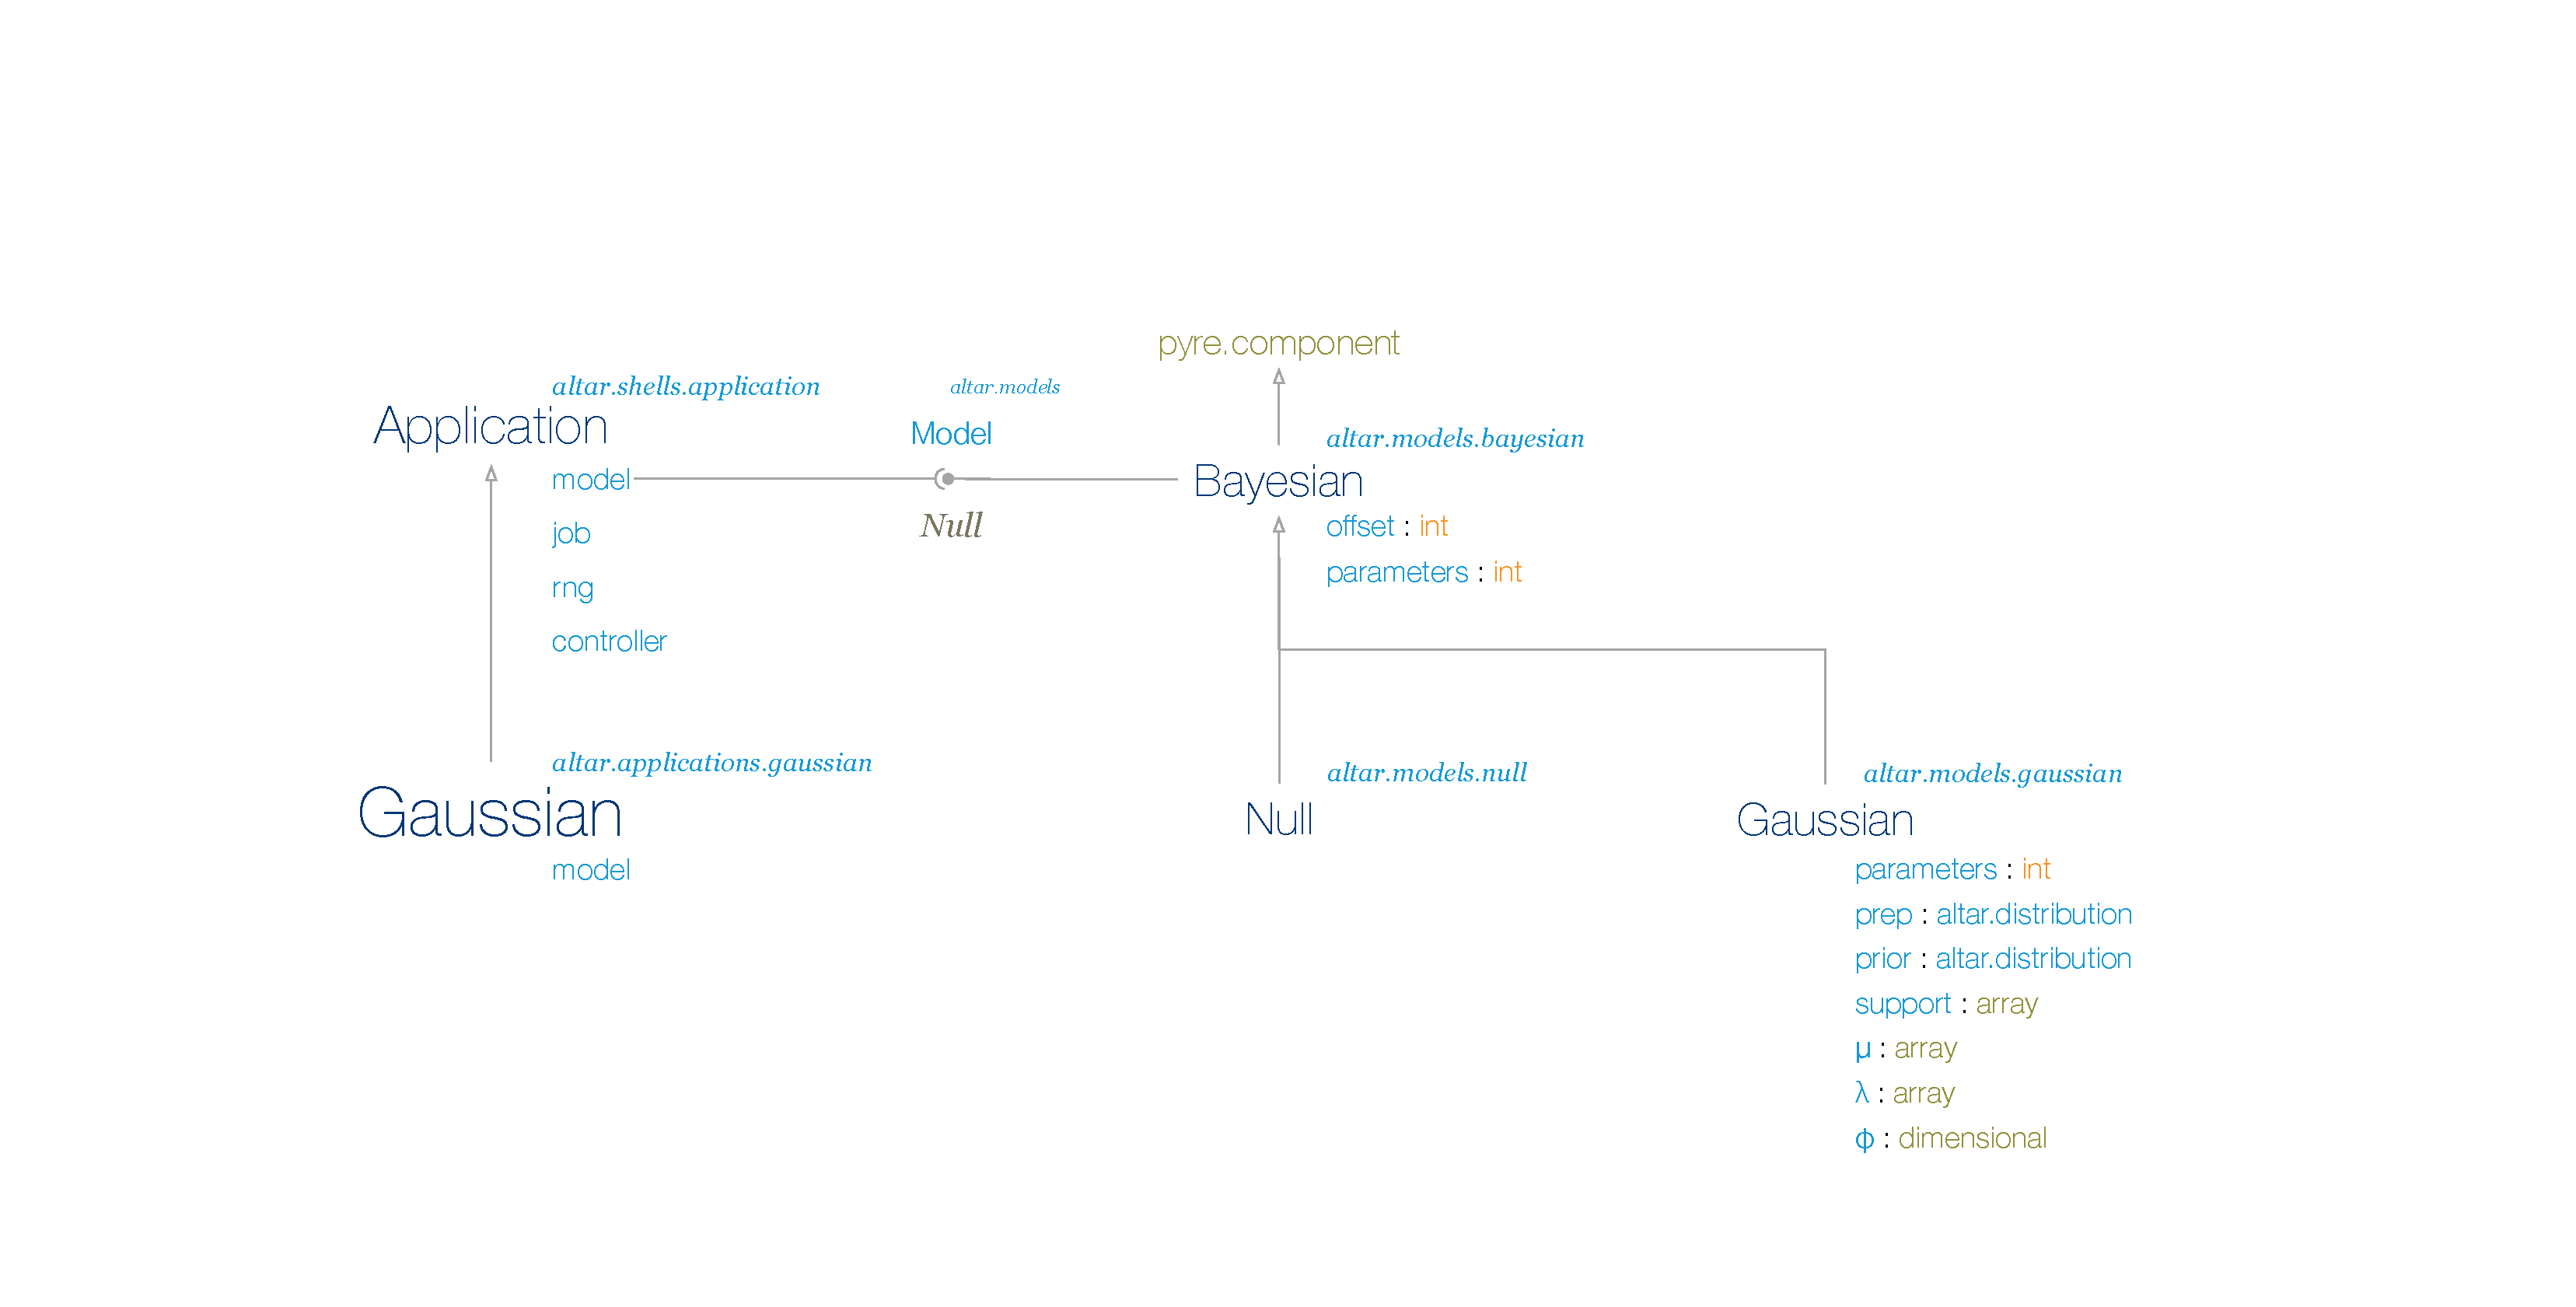
\includegraphics[width=1.0\textwidth]{application-model}
    \end{center}
  }
%
  \only<7>{
    \begin{center}
      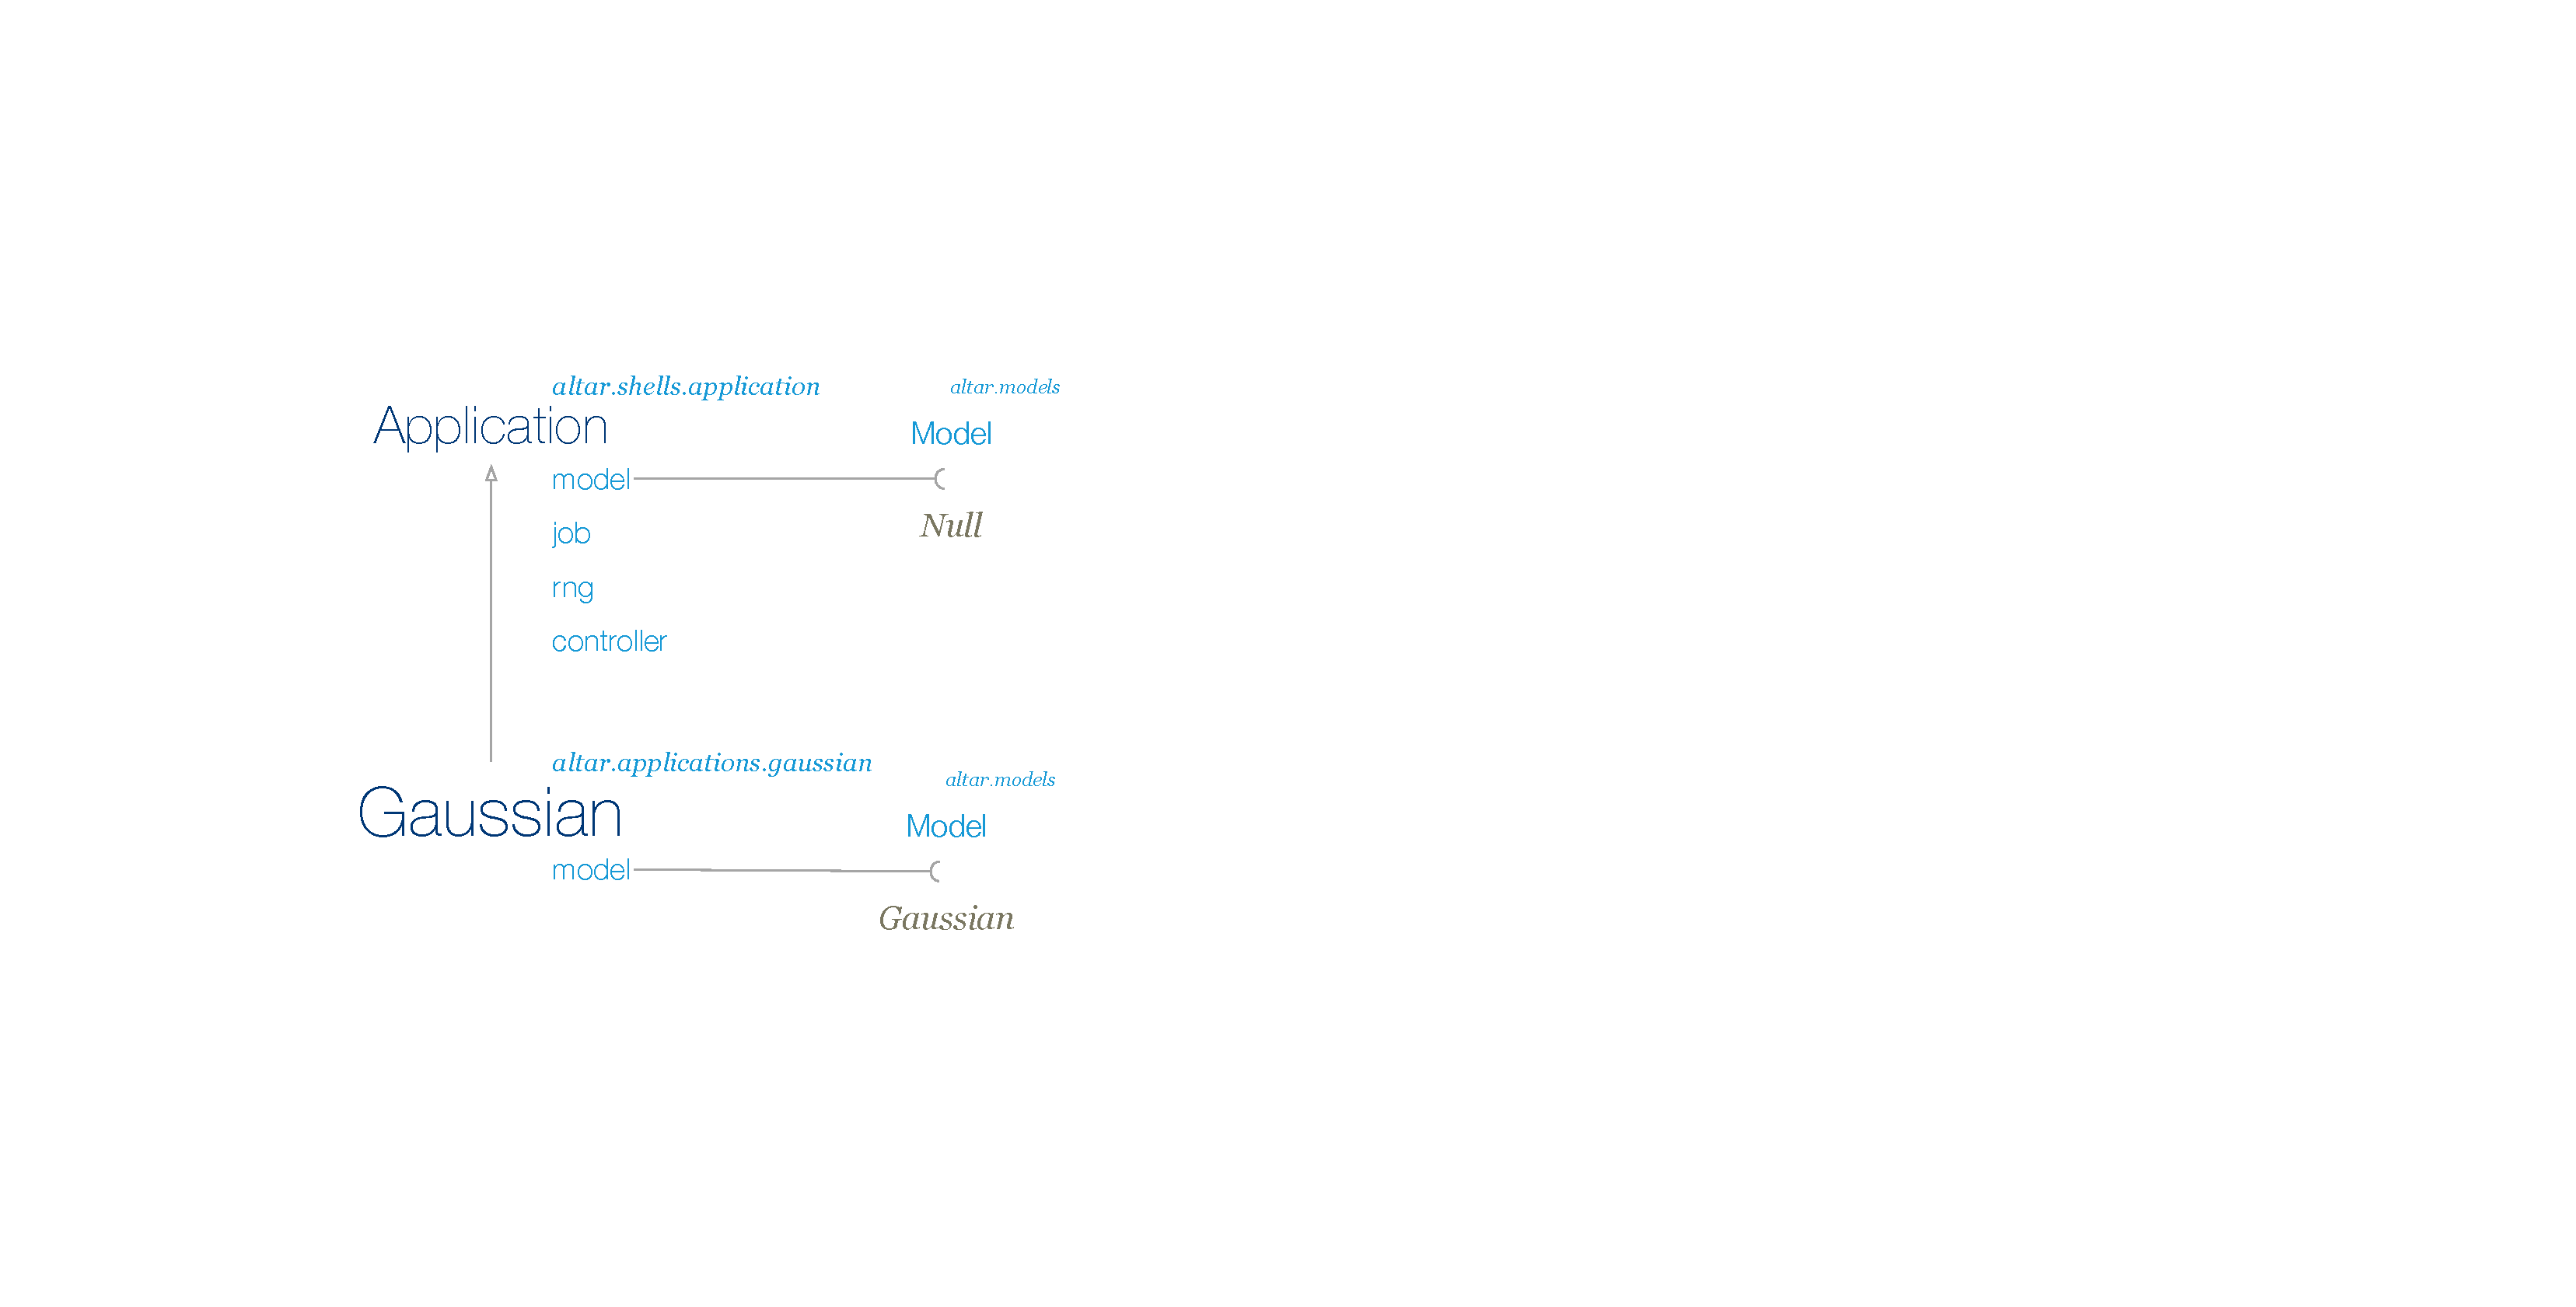
\includegraphics[width=1.0\textwidth]{application-model-override}
    \end{center}
  }
%
  \only<8>{
    \begin{center}
      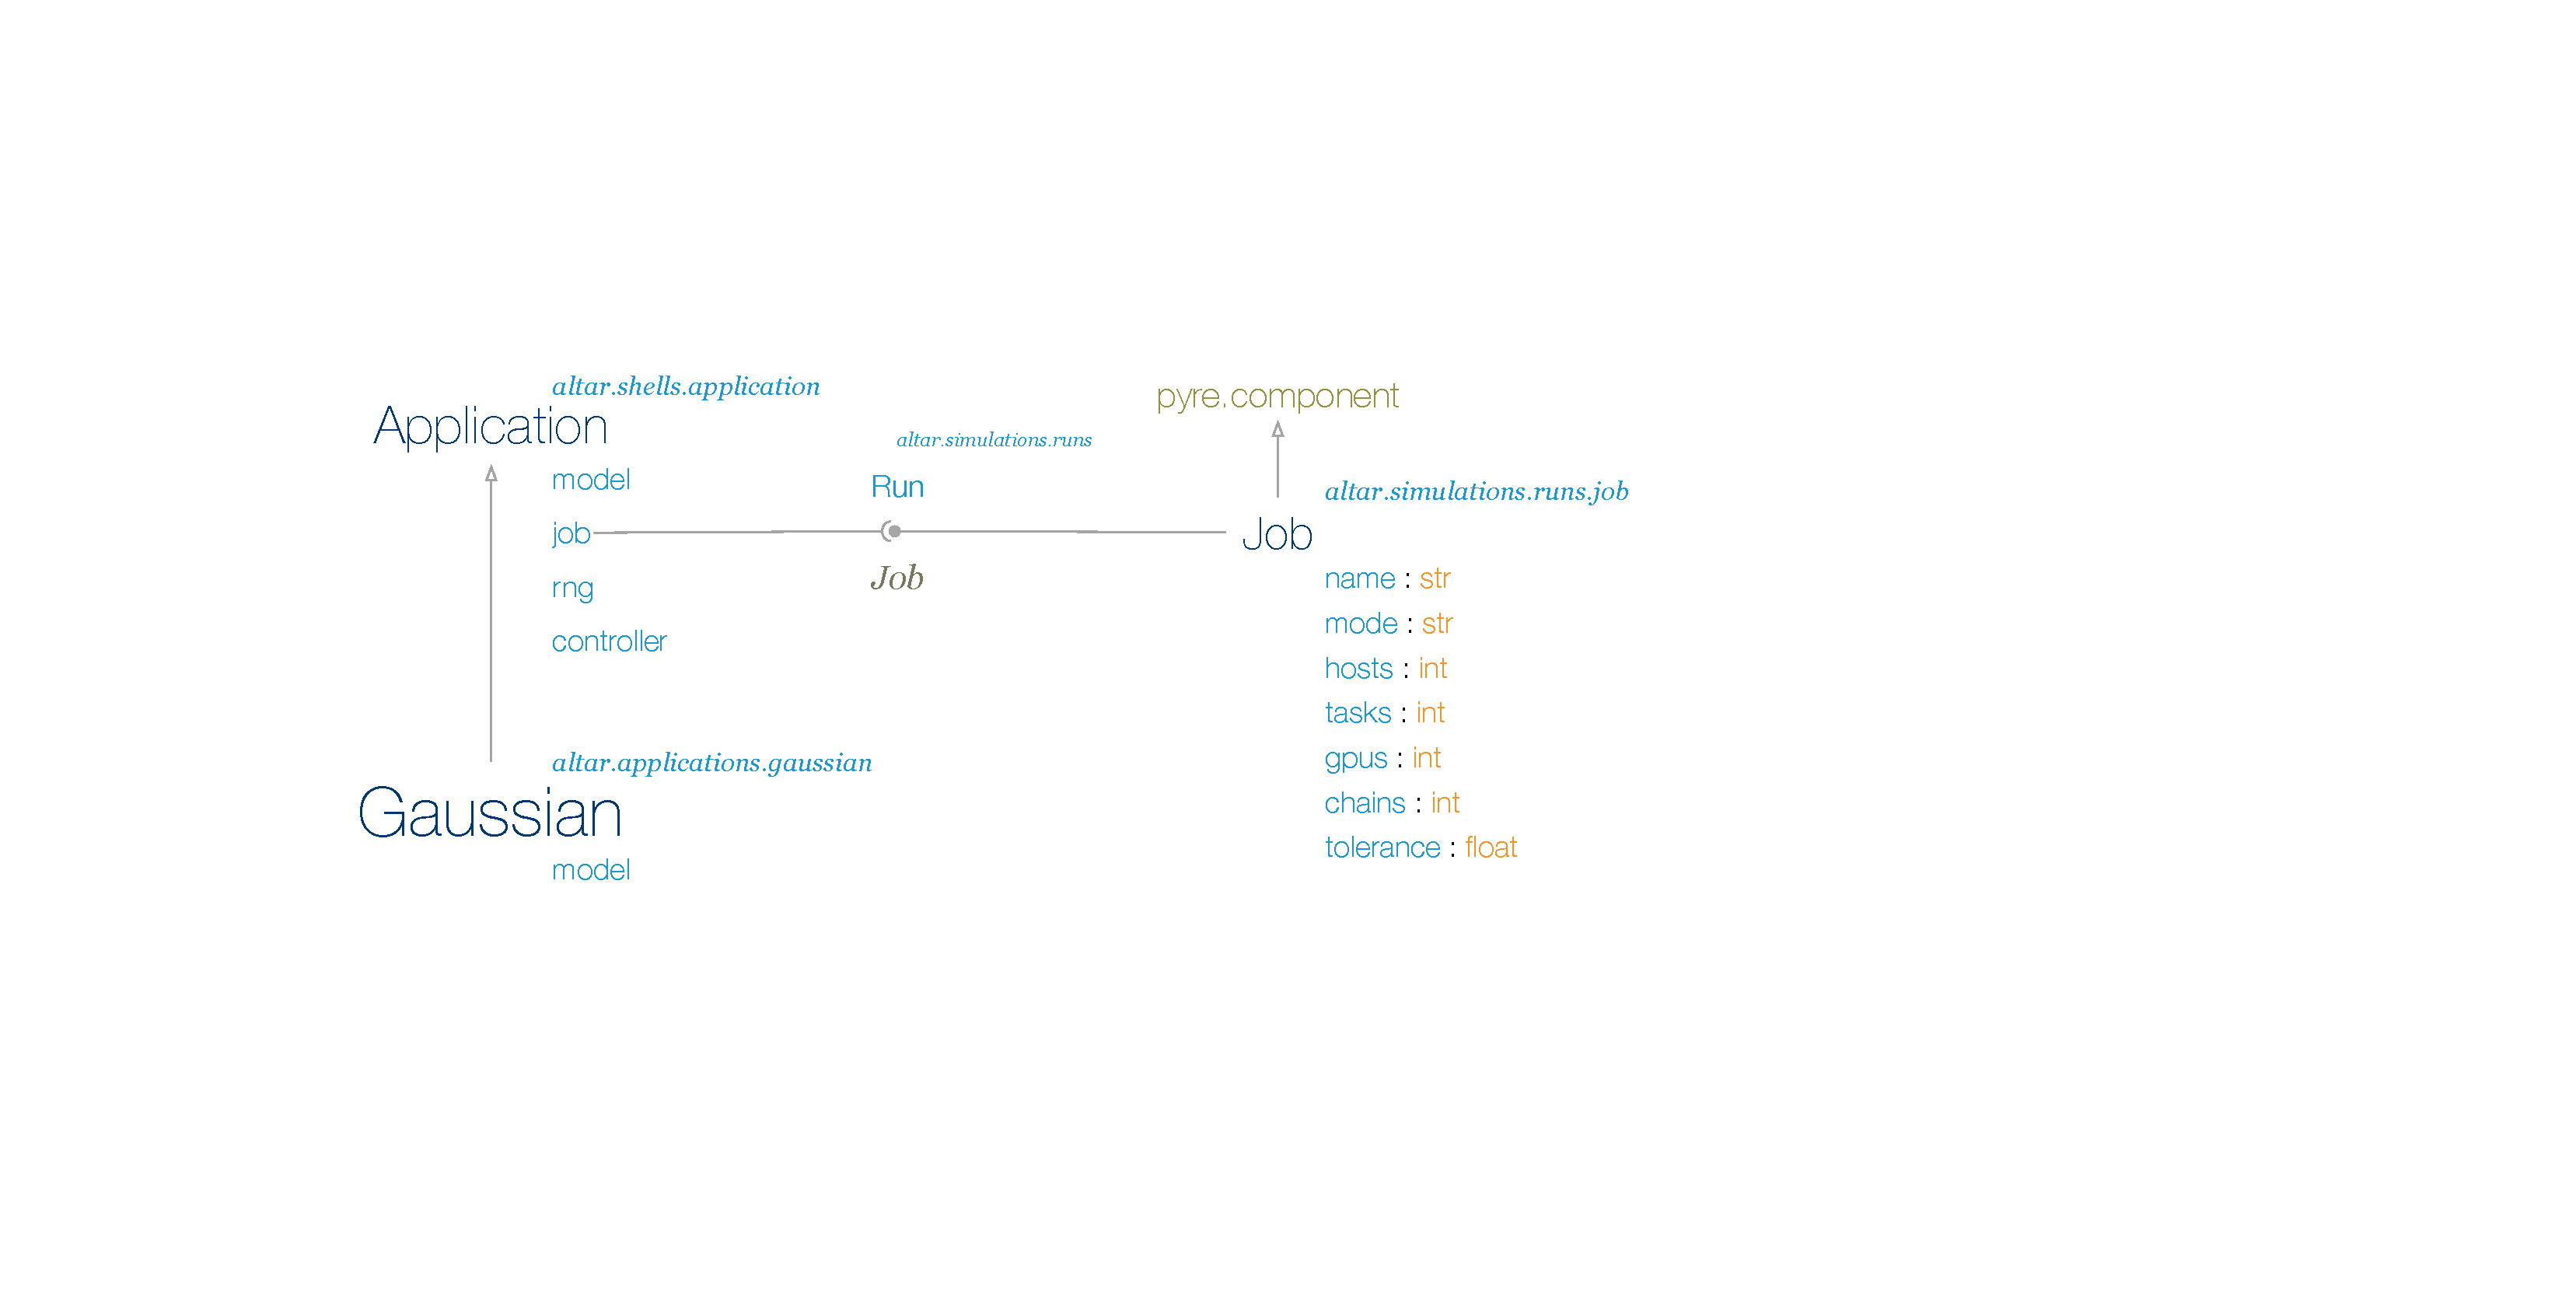
\includegraphics[width=1.0\textwidth]{application-job}
    \end{center}
  }
%
  \only<9>{
    \begin{center}
      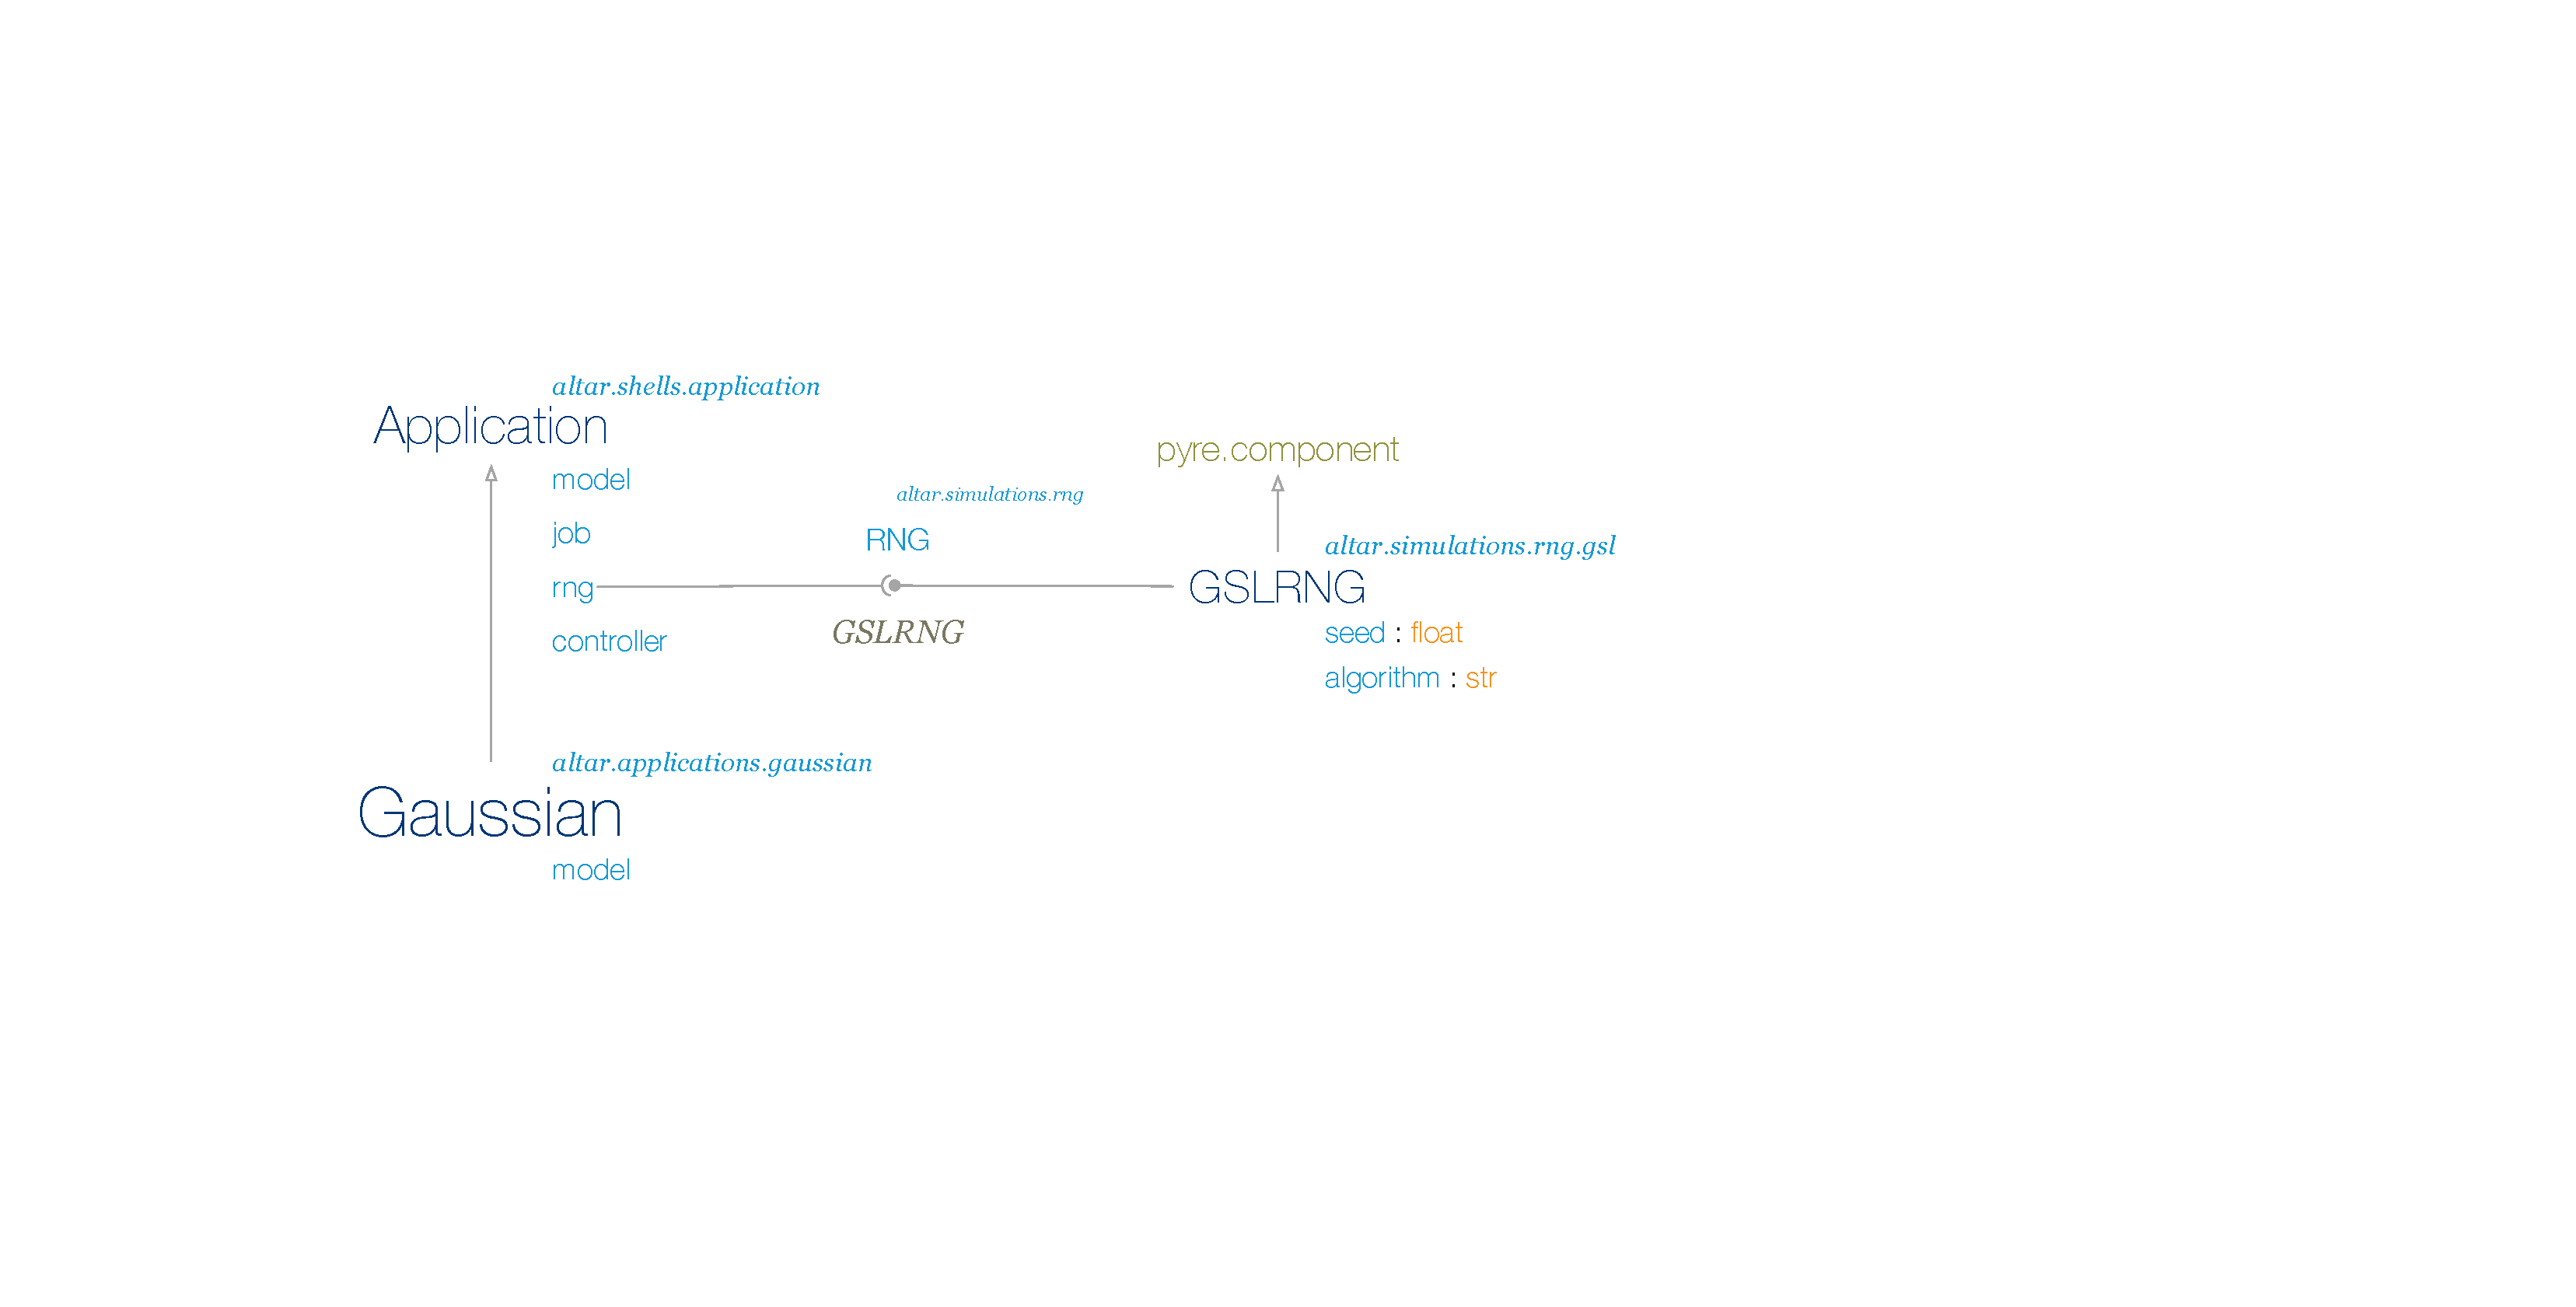
\includegraphics[width=1.0\textwidth]{application-rng}
    \end{center}
  }
%
  \only<10>{
    \begin{center}
      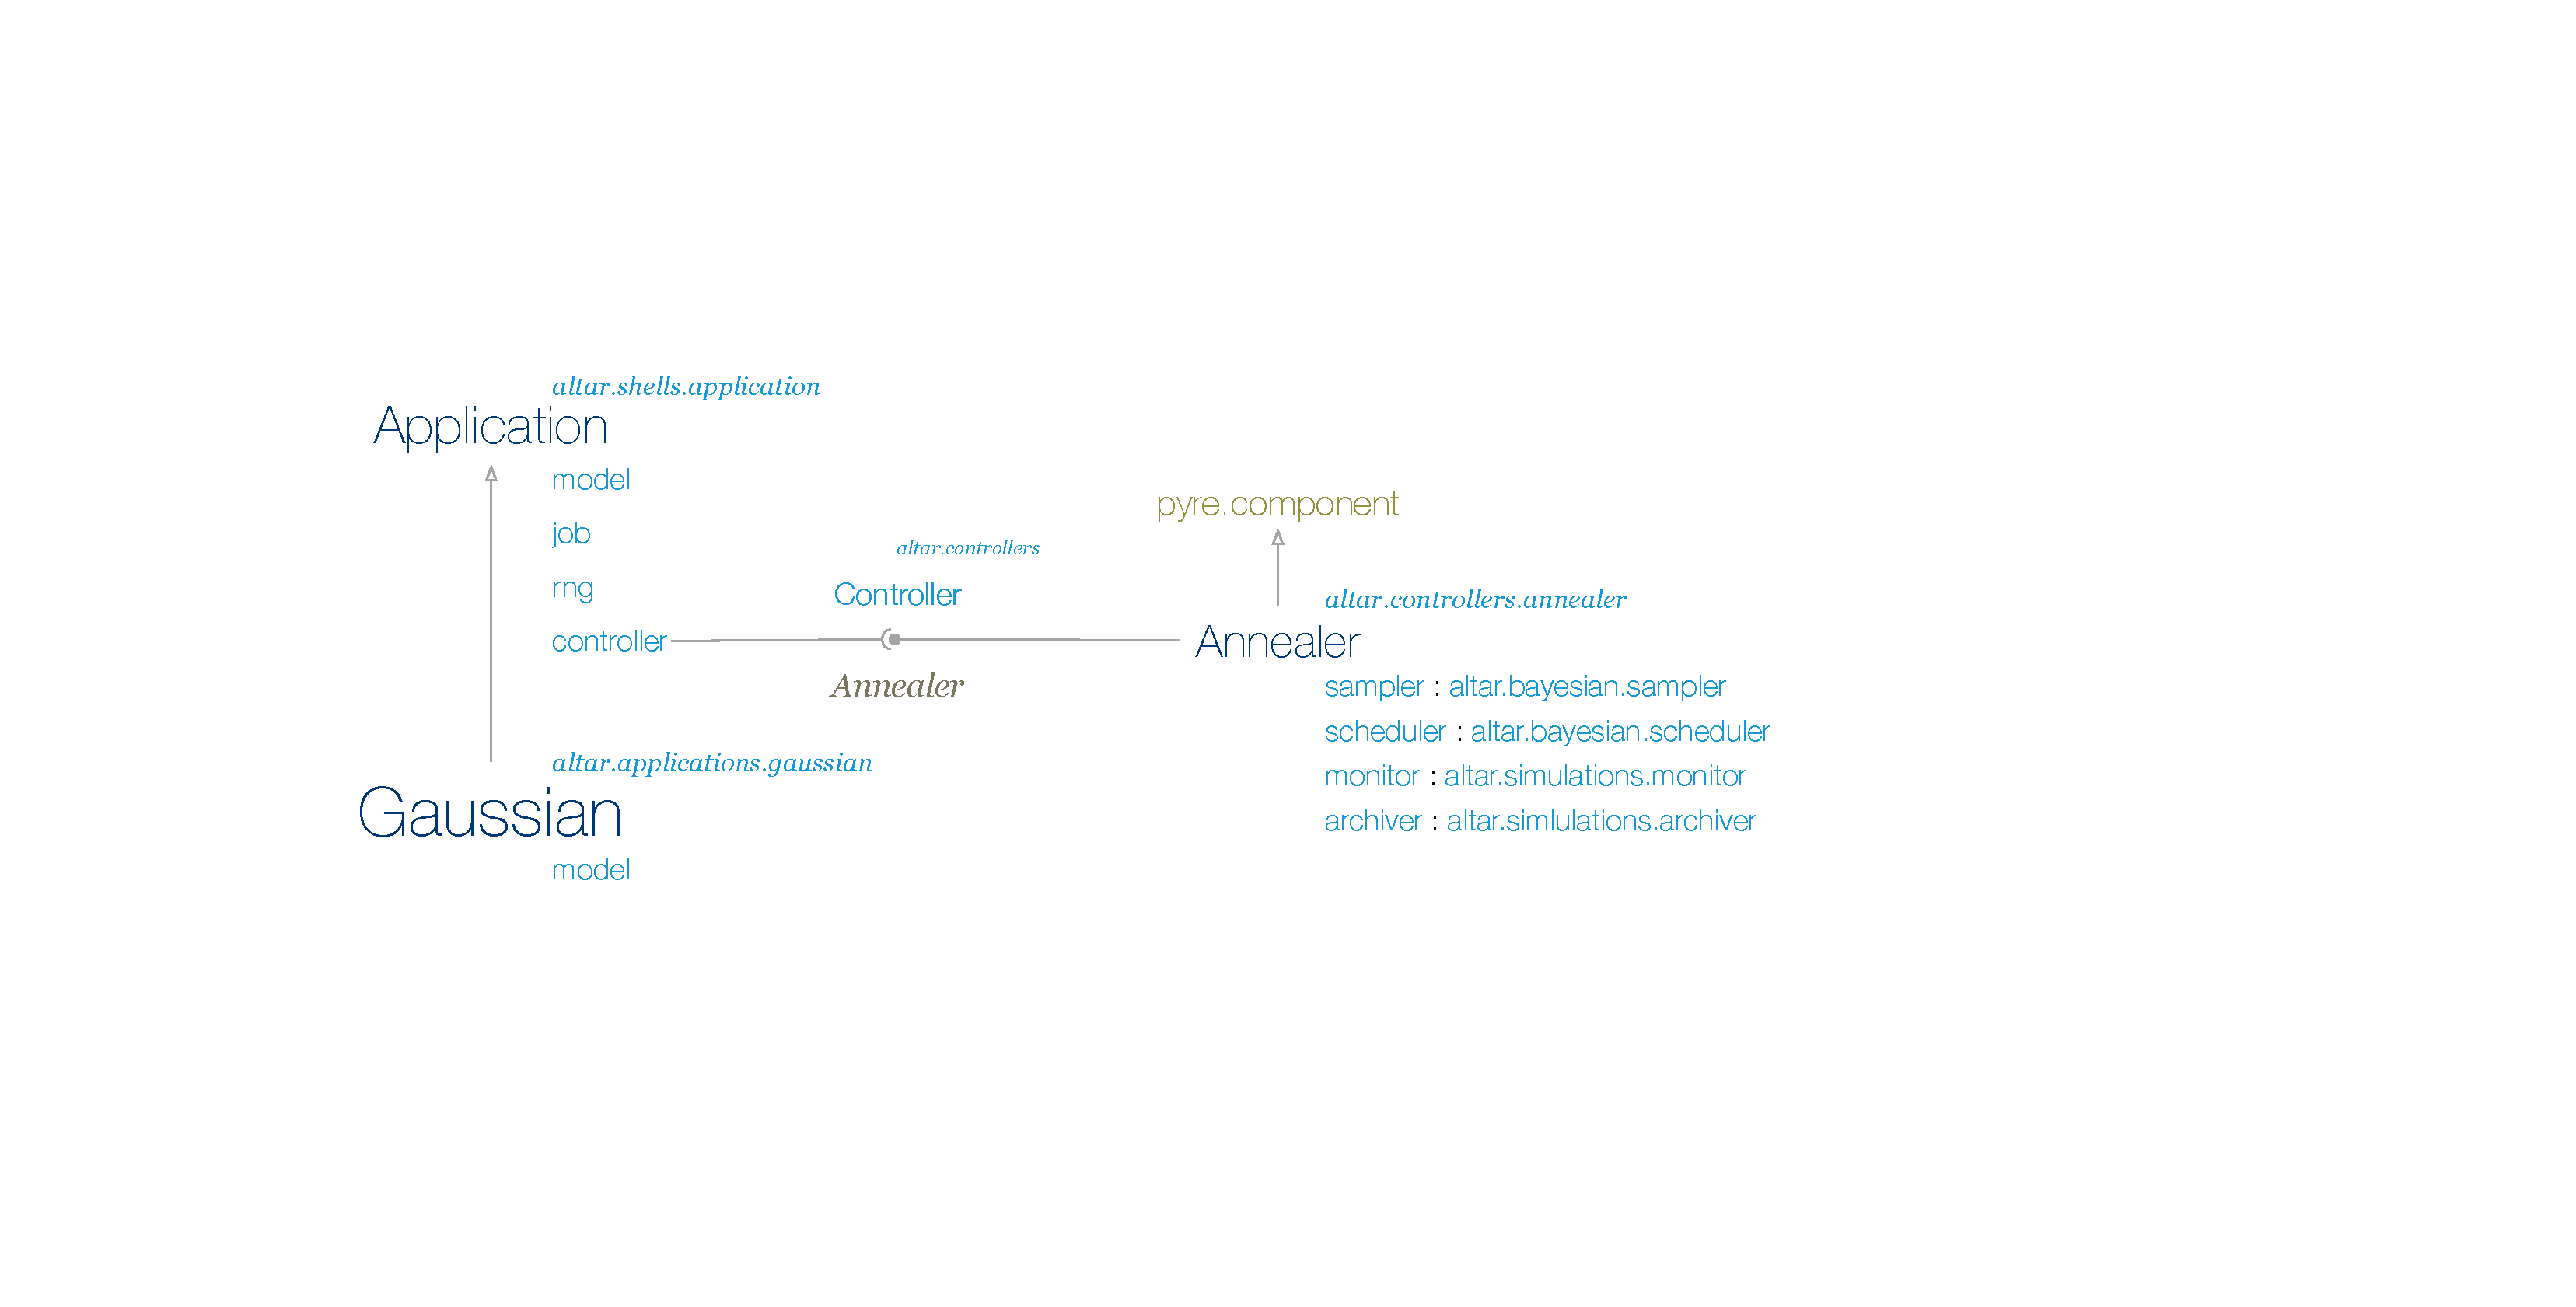
\includegraphics[width=1.0\textwidth]{application-controller}
    \end{center}
  }
%
\end{frame}

% end of file
